\documentclass[12pt]{../notes}

% Command for Questions
%\question{}

% Command for Notes
% \note{}

% Code to create a minipage where you can type in class notes. 
%%\begin{minipage}[l][2cm][c]{\textwidth}
%\begin{comment}

%\end{comment}
%%\end{minipage}

\usepackage{listings}

% In order for the minted code to run, we had to create a new compilation routine called pdflatex+shellEscape.
% This includes a --shell-escape command which should ONLY be used when pygmentized is required as it compromises security. 
% We also had to add pygmentize (a python package) to the system path (BEFORE miktex) and then restart the computer. 
\usepackage{minted}
\usemintedstyle{borland}
\lstset{language=SAS, 
  breaklines=true,  
  basicstyle=\ttfamily\bfseries,
  columns=fixed,
  keepspaces=true,
  identifierstyle=\color{blue}\ttfamily,
  keywordstyle=\color{cyan}\ttfamily,
  stringstyle=\color{purple}\ttfamily,
  commentstyle=\color{green}\ttfamily,
  } 
  
% \begin{minted}{sas}
% \end{minted}


% Begin Document
%==============================================================================
\begin{document}
% Include the Title of the Handout
\ntitle{2.3: Simple Model Inference}

Recall the simple linear model
\[
Y_i = \beta_0 + \beta_1X_{i,1} + \epsilon_i. 
\]

Inference is the process by which we make a decision about whether an observed difference from an expectation was simply due to chance or not. 

\nspace
In other words, inference is the process of making conclusions given incomplete information. 

% Include Numbered Sections
\section{Why Inference?}

Hypothetical questions:
\begin{itemize}
\item Suppose you found out that there is not significant relationship between study time and final grades in Stat 5100, how would this effect your approach to this course?
\item Suppose you have the flu and you find out from a clinical trial of a new flu drug that those who took the drug had slightly shorter flu durations than those who took the placebo, but that the difference was likely due to chance. How likely would you be to purchase this drug? 
\end{itemize}

\nspace
In the absence of complete information, inference is an efficient way to decide what associations are ``real'' and which are not.

\section{Hypothesis Testing}
Recall that hypothesis testing is the formal way by which we determine if an observed difference from an expectation was due to chance. 

\nspace
\subsection*{Process}
\bi
\item Define a null and alternative hypothesis. 
\bi
\item $H_0:$ ``no effect''
\item $H_a:$ ``some effect''
\ei
\item Define a test statistic:
\bi
\item Compares what we observed to what we expected if the null hypothesis was true. 
\ei
\item Determine the ``sampling distribution''
\bi
\item Determines the natural variation in the test statistic that we would expect if we took many different samples from the same population. 
\item In practice, we only ever take one sample. Statistical theory is what allows us to determine what the distribution would look like if we could take many samples. 
\item The distribution often relies on \textbf{model assumptions}. 
\ei
\item Get p-value
\bi
\item This is the probability of obtaining an observation as far, or farther, away from what we expected if the null was true. 
\ei
\item Make conclusion in context.
\bi
\item If the p-value is small ($<\alpha$), then it is unlikely that we would have obtained our observation if the null hypothesis is true. This provides evidence that the observed difference between our observation and expectation is REAL, and not simply due to chance. 
\ei
\ei

\subsection{Toluca Example:}
\textbf{If model assumptions are satisfied}, then $b_1 \sim N(\beta_1, \sigma^2\{b_1\})$.  

\begin{minipage}[l][2cm][c]{\textwidth}
%\begin{comment}
\note{$\sim$ means ``follows'' while $\sigma^2\{b_1\}$ represents the true variance of $b_1$, as estimated by $s\{b_1\}$.}
%\end{comment}
\end{minipage}

\nspace
Recall that, if the null hypothesis is true, then $\beta_1 = 0$. Thus, our test statistic becomes
\[
t = \frac{b_1 - 0}{s\{b_1\}} \sim t_{df_E} = 10.29
\]
with $25-2 = 23$ degrees of freedom with a \textbf{p-value $<$ 0.0001}.

\begin{minipage}[l][3cm][c]{\textwidth}
%\begin{comment}
\note{where $df_E$ is the degrees of freedom for the residuals, which is $n-2$ in the simple linear model case}

\nspace 

\note{draw t-distribution and shade the area that represents the p-value}
%\end{comment}
\end{minipage}

Since our p-value is lower than our level of significance (which is typically 0.05 and something we set beforehand), we would \textbf{reject} the null hypothesis \textbf{and conclude} that there is significant evidence that lot size and work hours are linearly related. 

\subsection*{Where did $\alpha = 0.05$ come from?}
Short answer: Sir Ronald Fisher, a prominent statistician, made it up:

\begin{quotation}
It is a common practice to judge a result significant, if it is such a magnitude that it would have been produced by chance not more frequently than once in twenty trials. This is an arbitrary, but convenient, level of significance for the practical investigator...\footnote{As on p99 of ``The Lady Tasting Tea'' (2001) by David Salsburg. See \url{http://jse.amstat.org/v16n2/velleman.pdf} for more discussion about statistical theory.}
\end{quotation}

However, $\alpha = 0.05$ has proven to be a good level of significance that balances the probability of Type I (claiming a difference when there isn't one) and Type II (claiming \textit{no} difference when there \textit{is} one). 


\subsection*{Consider the following}

You wish to determine if Aggie ice cream is more fattening than other ice cream shops in Logan. Suppose your null hypothesis is: ``Aggie ice cream has the same number of calories per cup as Charlie's ice cream.'' You then conduct a test and obtain a p-value of 0.048, indicating that there is evidence that the average caloric counts are significantly different. You then realize that you forgot to include five recorded observations in your study. When you include these additional observations, you obtain a p-value of 0.052, indicating no significant difference. 

\nspace
\textbf{P-values should inform an analysis, rather than become the analysis.}

\section*{Confidence Intervals}

\bi
\item General Form:
\[
\text{estimate} \pm (\text{critical value})\times(\text{SE of estimate})
\]
\item For $\beta_1$:
\[b_1 \pm t^*\times s\{b_1\}\]
\item Interpretation:
\bi
\item We are 95\% confident that the true value of $\beta_1$ is contained in this interval. 
\item If we were to create 100 confidence intervals from 100 different samples, we would expect about 95 of them to contain the true $\beta_1.$
\ei
\ei

\nspace
Testing $H_0: \beta_1$ at level $\alpha$ is the same as checking whether 0 is inside the $(1-\alpha)100\%$ CI for $\beta_1$. 

\section*{Model Inference}
All previous examples test whether an individual X variable has a significant linear relationship with Y. We will now look at some measures of model usefulness that apply when there is more than one $X$ variable. 

\subsection*{Ingredients of Model Inference}
\bi
\item Sum of Squares
\bi
\item $SS_{total} = \sum_i\left(Y_i - \bar{Y}\right)^2 \propto \text{variance of Y}$
\item $SS_{error} = \sum_i\left(Y_i - \hat{Y}_i\right)^2 = \sum_ie_i^2 \propto \text{variance not explained by model}$
\item $SS_{model} = SS_{total} - SS_{error}$
\ei
\ei

\begin{figure}[H]
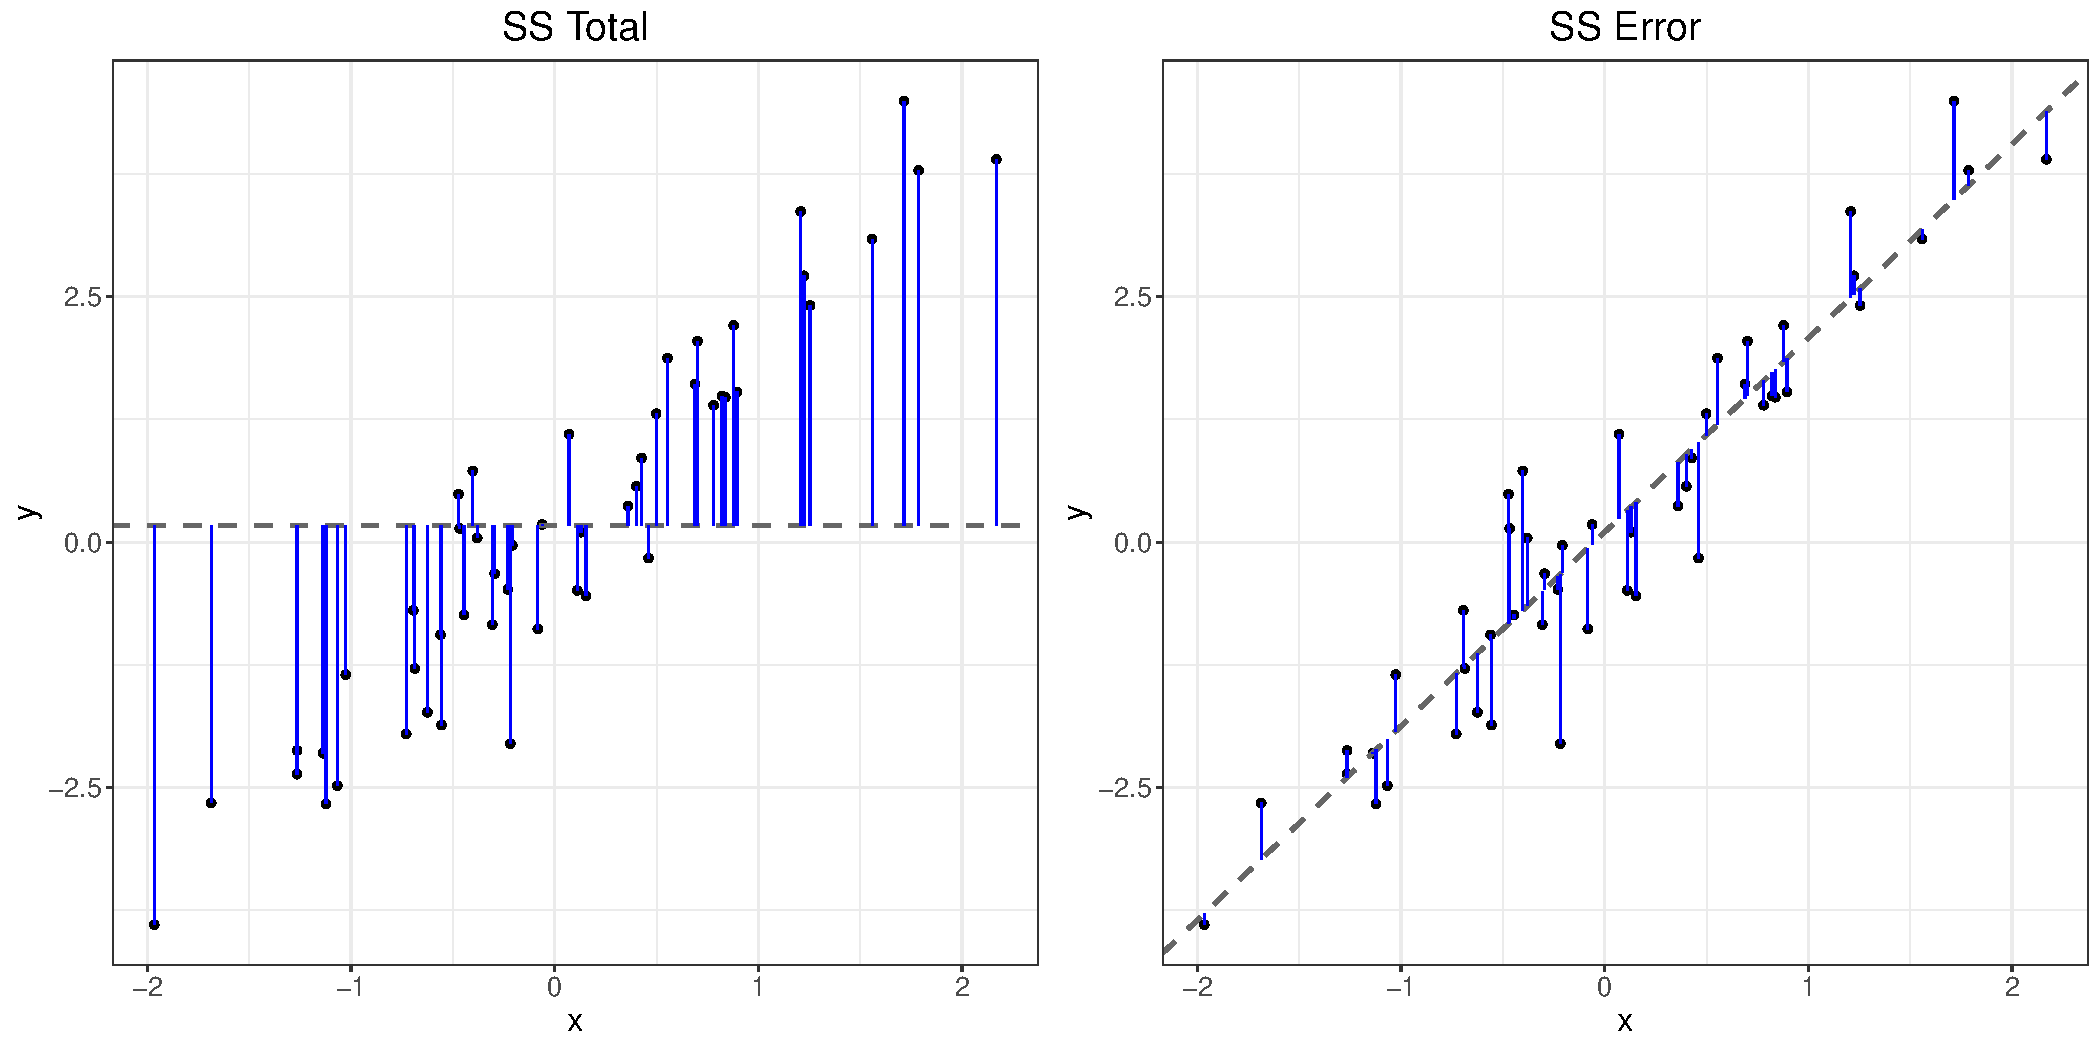
\includegraphics[width=\textwidth]{../figures/module2/ssError.pdf}
\caption{Illustration of $SS_{total}$ and $SS_{error}$.}
\end{figure}

\bi
\item Mean Square: $MS = \frac{SS}{df}$ 
\item $F = \frac{MS_{model}}{MS_{error}}$
\item $R^2 = \frac{SS_{model}}{SS_{total}} = 1 - \frac{SS_{error}}{SS_{total}}$
\bi
\item Interpretation: the percent of the variation in $Y$ that is explained by the model. 
\ei
\item MSE = Mean Square Error = $\hat{\sigma}^2$ = our best estimate of the error variance ($\epsilon \sim N(0, \sigma^2)$).
\ei

\subsection*{Toluca Example:}

\begin{minipage}[l][2cm][c]{\textwidth}
%\begin{comment}
\note{$R^2 = 0.82$ (from Handout 2.1.1) which means that about 82\% of the variation in work hours is explained by lot size.} 
%\end{comment}
\end{minipage}

Two other ways to look at $H_0: \beta_1 = 0:$

\begin{enumerate}
\item How much worse would the model fit be if we dropped the $\beta_1$ term?

Reduced Model (null hypothesis): $Y_i = \beta_0 + \epsilon_i$. 

Full Model: $Y_i = \beta_0 + \beta_1X_{i,1} + \epsilon_i$.

\nspace
F-statistic looks at chance in $SS_{error}$ between these two models. 

\nspace
Can be extended to consider removal of \textit{subsets} of $X$ variables (more later in the semester).  

\item Let $\rho = Corr(X,Y) = $ true, unknown correlation coefficient, which we estimate with the sample correlation $(r)$. 

\bi
\item When there is only one x-variable in the model it follows that 
\[H_0: \beta_1 = 0 \equiv H_0: \rho = 0.\]
\ei
\end{enumerate}

\section*{Inference on the Response Variable Y}
We can create interval estimates for the response variable. 

\[
\hat{Y} \pm t_{df_E}(1-\frac{\alpha}{2})*SE\{\hat{Y}\}
\]

Two Intervals:
\bi
\item \textbf{Confidence Interval}: Interval estimate of \textbf{mean} (or expected) Y for \textbf{population} of all $X = X_h.$
\[SE\{\hat{Y}\} = s\{\hat{Y}_h\} = \sqrt{\hat{\sigma}^2\left[\frac{1}{n} + \frac{(X_h - \bar{X})^2}{\sum_i (X_i - \bar{X})^2}\right]}\]
\item \textbf{Prediction Interval}: Interval estimate of \textbf{predicted} Y for a single [new] observation at $X = X_h$
\[SE\{\hat{Y}\} = s\{\hat{Y}_{h (new)}\} = \sqrt{\hat{\sigma}^2\left[1 + \frac{1}{n} + \frac{(X_h - \bar{X})^2}{\sum_i (X_i - \bar{X})^2}\right]}\]
\ei

\subsection*{Toluca Example (with $X_h = 10$)}
\bi
\item If we were to go to a new (single) lot of 10 acres, we are 95\% confident that the work hours would be between 
 
 \begin{minipage}[l][2cm][c]{\textwidth}
%\begin{comment}
\note{-13.6 (truncate at 0) and 209.7.} 
%\end{comment}
\end{minipage}

\item If we were to consider all possible 10 acre sized lots, we are 95\% confident that the mean work hours across all these lots would be between  

 \begin{minipage}[l][2cm][c]{\textwidth}
%\begin{comment}
\note{50.5 and 145.6.} 
%\end{comment}
\end{minipage}
\ei

\textbf{Note:} Most models have more than one predictor variable, we will use the following common notation throughout the remainder of this course:
\bi
\item $n =$ sample size
\item $p =$ number of $\beta_j$'s in the model (including the intercept)
\item $df_E = n-p$
\ei
















% End the Document
%==============================================================================
\end{document}